\section{Methodology}
	This chapter aims to detail the manner in which the experiments were carried out over the course of this project, as well their justification. Included in the chapter is information on how data was collected from task participants and the development of a system to process said data.

	\subsection{Collection of Dot-to-Dot Task Data}
		The core of this project was the analysis of MT data, which of course requires  the collection of said data. Ethical clearance was provided to allow the collection of data using the Dot-to-Dot Task from Edinburgh Napier University students and staff. After applying for and receiving ethical clearance for the collection and processing of Edinburgh Napier data, an email requesting volunteers was distributed to advertise the data collection process.
	
		Data collection took place on Edinburgh Napier University’s Merchiston campus, in the upstairs portion of a café. The environment in which the experiments were to take place was crucial to limit any possible distractions and ensure a fair trial for all participants. The location was well lit and had a low level of background noise. A desk and a chair were provided for participants, to ensure that the drawing tablet was at a comfortable height for use. 
	
		Before commencing the Dot-to-Dot Task, all test participants were asked to sign a wavier. This was to comply with the previously received ethical clearance and to ensure that the volunteer was content with collection and processing of their data and understood the reason for the collection of their data. This provided them with time to ask questions about the collection process and about the project as a whole. Prior to the meeting of volunteers, they were asked to provide some basic personal information, including their age, sex, dominant hand and Dyslexia Status - either Dyslexic, not Dyslexic or possibly Dyslexic. Ideally all participants would have been in either the Dyslexic or non-Dyslexic groups, but the possibly Dyslexic group was included to cater for volunteers who believed they portrayed Dyslexic tendencies, but had not had an official Dyslexia assessment. In total 76 individuals volunteered to participate in the project with 17 being Dyslexic, 31 being non-Dyslexic and 28 being possibly Dyslexic or unknown. Considering the national average of Dyslexia is 1:10, the turnout of Dyslexic participants compared to non-Dyslexic was extremely humbling.
	
		Each participant would complete a practice pattern before the task began properly. This was to familiarise them with using the stylus, a HCI input device that many of the volunteers were not accustomed to using on a regular basis. Once a participant completed the practice pattern, they were then tasked with completing pattern 3 and pattern 4 three times each. The task was performed two times, first with the individual's dominant hand and the second with their non-dominant hand. This resulted in a total of 14 patterns being drawn by each participant.
	
		The following script was read to task participants,\\
	
		‘The test begins when the stylus is in contact with the tablet and the cursor is moved to the starting position. If at any point you lift the stylus from the tablet, the test will be paused until the stylus is making contact with the tablet and you have moved the cursor back to the location from which you lifted it. The goal of the task is to move the cursor to target as quickly and accurately as you can. When the cursor gets close enough the target it will disappear and a new target will become visible.’\\
	
		The same script was used for every participant to ensure each individual began the task with the same information. The script was delivered while also demonstrating a sample Dot-to-Dot Task pattern, providing the subject with visual and vocal information of the task. 
	
		The Dot-to-Dot Task records data by login the X/Y position of the stylus, as well as a timestamp to a MySQL database. A data point is logged every time the X or Y coordinate of the stylus is updated. The system also logged when a task participant lifted the stylus from the drawing tablet. By recording the lifts, positional coordinates and timings of a Dot-to-Dot Task participant, it is possible to extrapolate all other required data that is required for Fitts’s Law analysis and thus, this project.
	
	\subsection{Data Processing System}
		Due to the sheer amount of data collected, a system was developed to automate the processing of said data, as well as to present it in a more usable format. A number of attractive options existed for the building of the processing system. In the end, Python was chosen as an appropriate language, thanks to its ability to allow for rapid prototyping as well as the mathematical and statistical libraries it provides.  Other options for tools or frameworks that could have been used include SQL and Groovy. However, Python was selected because...
		
		There existed a number of prerequisite stages to calculating an individual IP. These included calculating the ID for each Dot-to-Dot Task sector; performing regression analysis of the average MT and sector ID; and calculating individuals’ IP.
		
		\subsubsection{Calculating the Index of Difficulty}
			As previously stated, the ID of a movement is calculated as: \(ID = \log_2\left( \frac{2D}{W}\right)\).While the width of every target in the Dot-to-Dot Task is known -  a circle with a diameter of twenty pixels - the distances of each sector are not recorded in the database, only the X and Y coordinates of each target. Given the start and end coordinates of a line, its length can be calculated via Pythagorean theorem. Python’s inbuilt mathematics functions allowed for the simple calculation of a sector length once the coordinates were selected from the database.
			\\
			
			PRESENT TABLE OF IDS\\
			
			IMAGES OF IDS
			
			As can be seen, the ID varies very little over the course of either pattern, with the difference of difficulties for pattern 3 being  X and for pattern 4 Y.
			
		\subsubsection{Regression analysis}
			Once the Sector difficulties were calculated, it became possible to perform regression analysis. The exporting of relevant data, the MT averages and sector IDs of the sectors to csv format was a simple task for Python and allowed the data to be processed and plotted with tools such as R and Excel. 
			Fitts’s Law states that as the ID increases, so to does the MT, in a linear manner. This is visualised in [fig], the typically expected Fitts’s Law regression. The regression analysis of Patterns 3 and 4 [fig] produced entirely unexpected results, producing trend lines that bear no resemblance to the hypothesized Fitts’s model.
			There exists a number of possible reasons as to why the regression analysis trend lines were so unexpected. One likelihood is that it was caused by the lack of diversity in the sector IDs. Another possibility is that the non-uniform angles at which the lines had to be drawn affected the difficulty of the sector in ways that could not be measured by Fitts’s Law. A third potential explanation of the regression analysis results is the possibility that the continuous drawing of lines affected the MT - in most studies concerning Fitts’s Law, participants will draw a single line at a time, rather than in the Dot-to-Dot Task where several lines are drawn in succession. 
			
			\begin{figure}[]
				\centering
				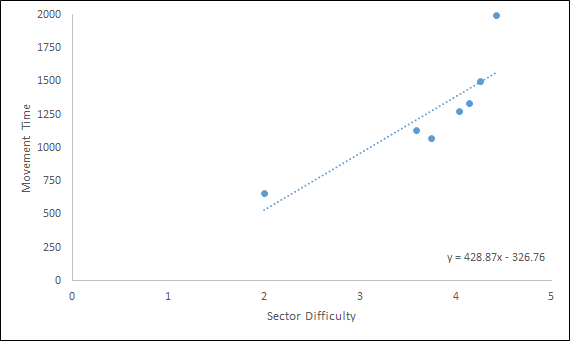
\includegraphics[width = \textwidth]{pat_3_reg}
				\caption{Regression Analysis of the Movement Times for Pattern 3 sectors.}
				\label{fig_pat_3_reg}
			\end{figure}
		
			\begin{figure}[]
				\centering
				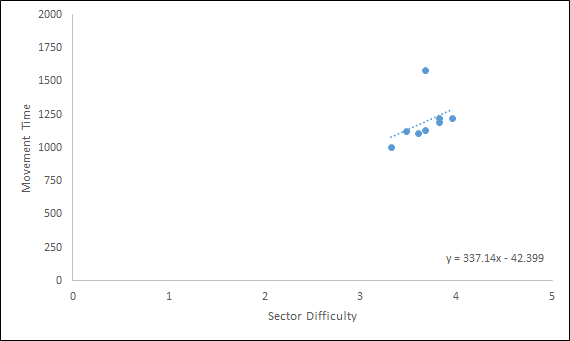
\includegraphics[width = \textwidth]{pat_4_reg}
				\caption{Regression Analysis of the Movement Times for Pattern 4 sectors.}
				\label{fig_pat_4_reg}
			\end{figure}
			
			\begin{table}[]
				\centering
				\caption{Pattern 3 - Regression Analysis input data.}
				\label{tab_pat_3_reg}
				\begin{tabular}{|c|c|}
					\hline
					\textbf{Sector ID} & \textbf{Movement Time} \\ \hline
					2.00               & 654.01                 \\ \hline
					3.59               & 1127.17                \\ \hline
					3.75               & 1073.18                \\ \hline
					4.04               & 1269.22                \\ \hline
					4.15               & 1334.30                \\ \hline
					4.26               & 1500.22                \\ \hline
					4.43               & 1991.61                \\ \hline
				\end{tabular}
			\end{table}
			
			\begin{table}[]
				\centering
				\caption{Pattern 4 - Regression Analysis input data}
				\label{tab_pat_4_reg}
				\begin{tabular}{|c|c|}
					\hline
					\textbf{Sector ID} & \textbf{Movement Time} \\ \hline
					3.32               & 1000.80                \\ \hline
					3.48               & 1119.50                \\ \hline
					3.61               & 1105.89                \\ \hline
					3.68               & 1584.11                \\ \hline
					3.68               & 1132.42                \\ \hline
					3.82               & 1219.60                \\ \hline
					3.82               & 1187.48                \\ \hline
					3.97               & 1216.46                \\ \hline
				\end{tabular}
			\end{table}
		
		\begin{table}[]
			\centering
			\caption{Pattern 3 - Average Movement Time in milliseconds for each sector.}
			\label{tab_pat_3_mt}
			\begin{tabularx}{\textwidth}{|r|r|X|X|X|X|X|X|X|}
				\hline
				\multicolumn{1}{|c|}{\textbf{Status}} & \multicolumn{1}{c|}{\textbf{Hand}} & \multicolumn{1}{c|}{\textbf{1}} & \multicolumn{1}{c|}{\textbf{2}} & \multicolumn{1}{c|}{\textbf{3}} & \multicolumn{1}{c|}{\textbf{4}} & \multicolumn{1}{c|}{\textbf{5}} & \multicolumn{1}{c|}{\textbf{6}} & \multicolumn{1}{c|}{\textbf{7}} \\ \hline
				Dyslexic                              & Dominant                           & 2054       & 1288       & 1157       & 680        & 1361       & 1539       & 1073       \\ \hline
				n-Dyslexic                          & Dominant                           & 1955       & 1258       & 1110       & 639        & 1319       & 1478       & 1074       \\ \hline
				Dyslexic                              & n-Dominant                            & 1972       & 1291       & 1125       & 683        & 1509       & 1419       & 1199       \\ \hline
				n-Dyslexic                          & n-Dominant                            & 1955       & 1387       & 1213       & 686        & 1511       & 1571       & 1256       \\ \hline
			\end{tabularx}
		\end{table}
			
		\begin{table}[]
			\centering
			\caption{Patter 4 - Average Movement Time in milliseconds for each sector.}
			\label{tab_pat_4_mt}
			\begin{tabularx}{\textwidth}{|r|r|X|X|X|X|X|X|X|X|}
				\hline
				\multicolumn{1}{|c|}{\textbf{Status}} & \multicolumn{1}{c|}{\textbf{Hand}} & \multicolumn{1}{c|}{\textbf{1}} & \multicolumn{1}{c|}{\textbf{2}} & \multicolumn{1}{c|}{\textbf{3}} & \multicolumn{1}{c|}{\textbf{4}} & \multicolumn{1}{c|}{\textbf{5}} & \multicolumn{1}{c|}{\textbf{6}} & \multicolumn{1}{c|}{\textbf{7}} & \multicolumn{1}{c|}{\textbf{8}} \\ \hline
				Dyslexic                              & Dominant                           & 1789       & 1205       & 1162       & 1145       & 1085       & 955        & 1233       & 1063       \\ \hline
				n-Dyslexic                          & Dominant                           & 1465       & 1228       & 1202       & 1125       & 1140       & 1027       & 1207       & 1131       \\ \hline
				Dyslexic                              & n-Dominant                       & 1426       & 1221       & 1272       & 1099       & 1177       & 1134       & 1427       & 1058       \\ \hline
				n-Dyslexic                          & n-Dominant                       & 1560       & 1245       & 1365       & 1225       & 1208       & 1080       & 1438       & 1245       \\ \hline
			\end{tabularx}
		\end{table}
	
			Regardless of the reasons, the results of the regression analysis were atypical to those that Fitts’s Law are normally expected to produce and a decision had to be made: either use the results of the regression analysis with the MacKenzie version of the equation as originally planned, or abandon the regression analysis and use the original Fitts’s equation of IP. Even though regression analysis is now the typically used method of Fitts’s Law analysis, it was opted that the original equation should be used over the MacKenzie version due to the unexpected nature of the regression analysis results.
			
		\subsubsection{Calculate Index of Performance}
			With the choice of performance equation decided, the final stage of development could begin. Using the original simplified equation made the calculation of an individual's performance a simple task of dividing a sector’s ID by the time taken for a participant to complete said sector. 
		
		\subsubsection{Exporting Results}
			Python is well renowned for the ease at which it can read, manipulate and export data. Using the Python csv libraries allowed data processed by the Fitts’s analysis to be quickly and simply converted and saved as csv file type. By saving results csv, it allowed data to be read and manipulated by a number of tools and frameworks including Microsoft Excel and R.
	
\newpage